\documentclass{beamer}
\usepackage{ctex}
\usepackage{minted}
\usepackage{smartdiagram}
\usetikzlibrary{positioning}
\usetheme{metropolis}           % Use metropolis theme
\title{Flink运行架构}
\date{\today}
\author{左元}
\institute{尚硅谷 大数据组}
\begin{document}
  \maketitle
  \begin{frame}
    \frametitle{主要内容}

    \begin{itemize}
        \item Flink运行时的组件
        \item 任务提交流程
        \item 任务调度原理
    \end{itemize}
  
  \end{frame}

  \begin{frame}
      \frametitle{Flink架构}
  
      \begin{itemize}
          \item Flink运行时由两种类型的进程组成:一个JobManager和一个或者多个TaskManager。
          \item 典型的Master-Slave架构。
      \end{itemize}
  
  \end{frame}

  \begin{frame}
    \frametitle{Flink架构}

    \begin{figure}
        \centering
        \scalebox{.8}{
            \begin{tikzpicture}
                \node[draw,circle,align=center](1){\large 作业管理器 \\ \large JobManager};
                \node[draw,circle,align=center](2)[above=of 1]{\tiny 任务管理器 \\ \tiny TaskManager};
                \node[draw,circle,align=center](3)[below=of 1]{\tiny 任务管理器 \\ \tiny TaskManager};
                \node[draw,circle,align=center](4)[left=of 1]{\tiny  任务管理器 \\ \tiny TaskManager};
                \node[draw,circle,align=center](5)[right=of 1]{\tiny 任务管理器 \\ \tiny TaskManager};
            \end{tikzpicture}
        }
        \caption{Flink架构}
    \end{figure}
  
  \end{frame}

  \begin{frame}
    \frametitle{作业管理器(JobManager)}

    \begin{itemize}
        \item 每个应用程序都会被一个不同的JobMaster所控制执行。
        \item JobManager会先接收到要执行的应用程序,这个应用程序会包括:作业图(JobGraph)、逻辑数据流图和打包了所有的类、库和其它资源的JAR包。
        \item JobManager会把JobGraph转换成一个物理层面的数据流图,这个图被叫做“执行图”(ExecutionGraph),包含了所有可以并发执行的任务。
        \item JobMaster会向资源管理器(Flink的资源管理器)请求执行任务必要的资源,也就是任务管理器(TaskManager)上的任务插槽(slot)。一旦它获取到了足够的资源,就会将执行图(DAG)分发到真正运行它们的TaskManager上。而在运行过程中,JobManager会负责所有需要中央协调的操作,比如说检查点(checkpoints)的协调。
    \end{itemize}
  
  \end{frame}

  \begin{frame}
    \frametitle{作业管理器(JobManager)}

    \begin{itemize}
        \item 资源管理器(ResourceManager):ResourceManager 负责 Flink 集群中的资源提供、回收、分配 - 它管理task slots,这是Flink集群中资源调度的单位。Flink为不同的环境和资源提供者(例如YARN、Mesos、Kubernetes和standalone部署)实现了对应的ResourceManager。在standalone设置中,ResourceManager只能分配可用TaskManager的slots,而不能自行启动新的TaskManager。
        \item 分发器(Dispatcher):Dispatcher 提供了一个 REST 接口,用来提交 Flink 应用程序执行,并为每个提交的作业启动一个新的 JobMaster。它还运行 Flink WebUI 用来提供作业执行信息。
        \item JobMaster:JobMaster负责管理单个JobGraph的执行。Flink集群中可以同时运行多个作业,每个作业都有自己的JobMaster。
    \end{itemize}
  
  \end{frame}

  \begin{frame}
      \frametitle{资源管理器}
  
      \begin{itemize}
          \item 主要负责管理任务管理器(TaskManager)的插槽(slot),TaskManager 插槽是Flink中定义的处理资源单元。
          \item Flink为不同的环境和资源管理工具提供了不同资源管理器,比如YARN、Mesos、Kubernetes(管理docker容器组成的集群),以及Standalone(独立集群)部署。
          \item 当JobManager申请插槽资源时,Flink的资源管理器会将有空闲插槽的TaskManager分配给JobManager。如果Flink的资源管理器没有足够的插槽来满足JobManager的请求,它还可以向Yarn的资源管理器发起会话,以提供启动TaskManager进程的容器。
      \end{itemize}
  
  \end{frame}

  \begin{frame}
      \frametitle{分发器}
  
      \begin{itemize}
          \item 可以跨作业运行,它为应用提交提供了RESTful接口(GET/PUT/DELETE/POST)。
          \item 当一个应用被提交执行时,分发器就会启动并将应用移交给一个JobManager。
          \item Dispatcher也会启动一个Web UI(localhost:8081),用来方便地展示和监控作业执行的信息。
          \item Dispatcher在架构中可能并不是必需的,这取决于应用提交运行的方式。
      \end{itemize}
  
  \end{frame}

  \begin{frame}
      \frametitle{任务提交流程}
  
      \begin{figure}
        \centering
        \scalebox{.8}{
            \begin{tikzpicture}
                \filldraw[fill=blue!40!white, draw=black] (-2,2) rectangle (0,2.4) node[pos=.5] {\tiny{App}};
                
                \filldraw[fill=blue!40!white, draw=black] (-2,0) rectangle (0,0.4) node[pos=.5] {\tiny{Dispatcher}};
                
                \filldraw[fill=blue!40!white, draw=black] (2,2) rectangle (4,2.4) node[pos=.5] {\tiny{ResoureManager}};
                
                \filldraw[fill=blue!40!white, draw=black] (2,0) rectangle (4,0.4) node[pos=.5] {\tiny{JobManager}};
                
                \filldraw[fill=blue!40!white, draw=black] (4.8,1.2) rectangle (6.8,1.6);
                \filldraw[fill=blue!40!white, draw=black] (4.9,1.1) rectangle (6.9,1.5);
                \filldraw[fill=blue!40!white, draw=black] (5,1) rectangle (7,1.4) node[pos=.5] {\tiny{TaskManager}};
                
                \draw[->] (7,1.4) to[out=60,in=30] (6.9,1.5);
                \draw[->] (6.9,1.5) to[out=60,in=30] (6.8,1.6);
                
                \draw[->] (-1,2) -- (-1,0.4);
                \draw[<-] (3,2) -- (3,0.4);
                \draw[->] (0,0.2) -- (2,0.2);
                \draw[->] (4,0.4) -- (5,1);
                \draw[<-] (4,0.2) -- (5.3,1);
                \draw[<-] (4,2.2) -- (4.8,1.6);
                \draw[->] (4,2.4) -- (5.1,1.6);
                
                \node[text width=2cm] at (-1.2,1.2) {\tiny{提交应用}};
                \node[text width=2cm] at (2.6,1.2) {\tiny{请求slots}};
                \node[text width=2cm] at (1.3,0.05) {\tiny{启动并提交应用}};
                \node[text width=2cm] at (8.05,1.4) {\tiny{交换数据}};
                
                \draw[->,dash dot,red] (4.2,0.52) -- (4.2,-0.5);
                \node[text width=4cm] at (4.2,-0.7) {\tiny{提交要在slots中执行的任务}};
                \draw[->,dash dot,red] (4.8,0.62) -- (5.8,-0.2);
                \node[text width=2cm] at (6.8,-0.2) {\tiny{提交slots}};
                
                \draw[->,dash dot,red] (4.3,2) -- (5.4,3);
                \draw[->,dash dot,red] (5,1.8) -- (6,2.4);
                \node[text width=2cm] at (6,3.2) {\tiny{注册slots}};
                \node[text width=3cm] at (7.4,2.5) {\tiny{发出提供slots的指令}};
            \end{tikzpicture}
        }
        \caption{Flink任务提交流程}
    \end{figure}
  
  \end{frame}

  \begin{frame}
      \frametitle{任务调度原理}

      \begin{figure}
        \centering
        \includegraphics[height=0.6\textheight]{image13.pdf}
        \caption{Flink运行时的组件}
      \end{figure}
  
  \end{frame}

  \begin{frame}
      \frametitle{TaskManager和Slots}

      \begin{figure}
        \centering
        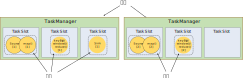
\includegraphics[width=0.6\textwidth]{tasks_slots.pdf}
        \caption{任务管理器和插槽}
      \end{figure}
  
      \begin{itemize}
          \item Flink 中每一个 TaskManager 都是一个JVM进程,每一个任务插槽都会启动一个线程,它可能会在独立的线程上执行一个或多个 subtask,每一个子任务占用一个任务插槽(Task Slot)
          \item 为了控制一个TaskManager能接收多少个task,TaskManager通过task slot来进行控制(一个TaskManager至少有一个slot)
      \end{itemize}
  
  \end{frame}

  \begin{frame}
      \frametitle{TaskManager和Slots}
  
      \begin{itemize}
          \item 默认情况下,Flink允许子任务共享slot。这样的结果是,一个slot可以保存作业的整个管道。
          \item Task Slot是静态的概念,是指TaskManager具有的并发执行能力。
      \end{itemize}
  
  \end{frame}

  \begin{frame}
      \frametitle{TaskManager和Slots}
  
      \begin{figure}
        \centering
        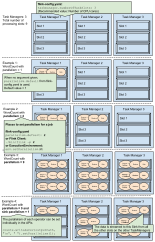
\includegraphics[height=0.6\textheight]{slots_parallelism.pdf}
        \caption{并行度}
      \end{figure}
  
  \end{frame}

  \begin{frame}
      \frametitle{程序与数据流(DataFlow)}
  
      \begin{figure}
          \centering
          \includegraphics[height=0.4\textheight]{program_dataflow.pdf}
          \caption{数据流}
      \end{figure}

      \begin{itemize}
          \item 所有的Flink程序都是由三部分组成的:Source、Transformation和Sink。
          \item Source负责读取数据源,Transformation利用各种算子进行处理加工,Sink负责输出。
      \end{itemize}
  
  \end{frame}

  \begin{frame}
      \frametitle{程序与数据流(DataFlow)}

      \begin{itemize}
          \item 在运行时,Flink上运行的程序会被映射成“逻辑数据流”(dataflows),它包含了这三部分
          \item 每一个dataflow以一个或多个sources开始以一个或多个sinks结束。dataflow类似于任意的有向无环图(DAG)
          \item 在大部分情况下,程序中的转换运算(transformations)跟dataflow中的算子(operator)是一一对应的关系
      \end{itemize}

      \begin{figure}
          \centering
          \includegraphics[width=0.6\textwidth]{image21.png}
          \caption{数据流}
      \end{figure}
  
  \end{frame}

  \begin{frame}
      \frametitle{图数据结构的转化}

      \begin{center}
        \smartdiagramset{
            border color=none,
            set color list={blue!50!cyan,green!60!lime,orange!50!red,red!80!black},
            back arrow disabled=true
        }
        \smartdiagram[flow diagram:horizontal]{StreamGraph, JobGraph, ExecutionGraph, 物理执行图}
      \end{center}

      \begin{itemize}
          \item StreamGraph:是根据用户通过 Stream API 编写的代码生成的最初的图。用来表示程序的拓扑结构。
          \item JobGraph:StreamGraph在编译的阶段经过优化后生成了 JobGraph,提交给 JobManager 的数据结构。主要的优化为,将多个符合条件(窄依赖,没有shuffle)的算子 chain 在一起作为一个节点。
          \item ExecutionGraph:JobManager 根据 JobGraph 生成ExecutionGraph。ExecutionGraph是JobGraph的并行化版本,是调度层最核心的数据结构。
          \item 物理执行图:JobManager 根据 ExecutionGraph 对 Job 进行调度后,在各个TaskManager 上部署 Task 后形成的“图”,并不是一个具体的数据结构。
      \end{itemize}
  
  \end{frame}

  \begin{frame}
      \frametitle{图数据结构的转化}
  
      \begin{figure}
        \centering
        \includegraphics[height=0.6\textheight]{flink_graph.png}
        \caption{图的转化}
      \end{figure}
  
  \end{frame}

  \begin{frame}
      \frametitle{并行度(Parallelism)}
  
      \begin{figure}
        \centering
        \includegraphics[height=0.4\textheight]{parallel_dataflow.pdf}
        \caption{图的转化}
      \end{figure}

      \begin{itemize}
          \item 一个特定算子的子任务(subtask)的个数被称之为其并行度(parallelism)。一般情况下,一个 stream 的并行度,可以认为就是其所有算子中最大的并行度。
      \end{itemize}
  
  \end{frame}

  \begin{frame}
      \frametitle{并行度(Parallelism)}
  
      \begin{itemize}
          \item 一个程序中,不同的算子可能具有不同的并行度
          \item 算子之间传输数据的形式可以是 one-to-one (forwarding) 的模式也可以是redistributing 的模式,具体是哪一种形式,取决于算子的种类
          \begin{itemize}
              \item One-to-one:stream维护着分区以及元素的顺序(比如source和map之间)。这意味着map 算子的子任务看到的元素的个数以及顺序跟 source 算子的子任务生产的元素的个数、顺序相同。map、filter、flatMap等算子都是one-to-one的对应关系。
              \item Redistributing:stream的分区会发生改变。每一个算子的子任务依据所选择的transformation发送数据到不同的目标任务。例如,keyBy 基于 hashCode 重分区、而 broadcast 和 rebalance 会随机重新分区,这些算子都会引起redistribute过程,而 redistribute 过程就类似于 Spark 中的 shuffle 过程。
          \end{itemize}
      \end{itemize}
  
  \end{frame}

  \begin{frame}
      \frametitle{任务链(Operator Chains)}
  
      \begin{itemize}
          \item Flink 采用了一种称为任务链的优化技术,可以在特定条件下减少本地通信的开销。为了满足任务链的要求,必须将两个或多个算子设为相同的并行度,并通过本地转发(local forward)的方式进行连接
          \item 相同并行度的 one-to-one 操作,Flink 这样相连的算子链接在一起形成一个 task,原来的算子成为里面的 subtask
          \item 并行度相同、并且是 one-to-one 操作,两个条件缺一不可
      \end{itemize}
  
  \end{frame}

  \begin{frame}
      \frametitle{并行度(Parallelism)}

      \begin{figure}
        \centering
        \includegraphics[width=0.9\textwidth]{image15.png}
        \caption{并行度}
      \end{figure}
      
  \end{frame}

  \begin{frame}
      \frametitle{任务链}
  
      \begin{figure}
        \centering
        \includegraphics[height=0.6\textheight]{operator_chaining.png}
        \caption{任务链}
      \end{figure}      
  
  \end{frame}

  \begin{frame}[plain,c]
    %\frametitle{A first slide}
    
    \begin{center}
    \Huge Q \& A
    \end{center}
    
  \end{frame}

\end{document}
